\documentclass{beamer}
\usepackage[utf8]{inputenc}
\usepackage{graphicx, epsfig}
\usepackage{amsmath,mathrsfs,amsfonts,amssymb}
\usepackage{floatflt}
\usepackage{epic,ecltree}
\usepackage{mathtext}
\usepackage{fancybox}
\usepackage{fancyhdr}
\usepackage{multirow}
\usepackage{enumerate}
\usepackage{epstopdf}
\usepackage{multicol}
\usepackage{algorithm}
\usepackage[noend]{algorithmic}
\usepackage{tikz}
\usepackage{blindtext}
\usetheme{default}%{Singapore}%{Warsaw}%{Warsaw}%{Darmstadt}
\usecolortheme{default}

\setbeamerfont{title}{size=\Huge}
\setbeamertemplate{footline}[page number]{}

\setbeamertemplate{section in toc}[sections numbered]


\makeatletter
\newcommand\HUGE{\@setfontsize\Huge{35}{40}}
\makeatother    

\setbeamerfont{title}{size=\HUGE}
\beamertemplatenavigationsymbolsempty

% latin bold lower
\newcommand{\ba}{\mathbf{a}} 
\newcommand{\bc}{\mathbf{c}} 
\newcommand{\be}{\mathbf{e}} 
\newcommand{\bh}{\mathbf{h}} 
\newcommand{\bp}{\mathbf{p}} 
\newcommand{\bt}{\mathbf{t}} 
\newcommand{\bs}{\mathbf{s}} 
\newcommand{\bu}{\mathbf{u}} 
\newcommand{\bv}{\mathbf{v}} 
\newcommand{\bw}{\mathbf{w}} 
\newcommand{\bx}{\mathbf{x}} 
\newcommand{\by}{\mathbf{y}} 
\newcommand{\bz}{\mathbf{z}} 

% latin bold upper
\newcommand{\bA}{\mathbf{A}} 
\newcommand{\bB}{\mathbf{B}} 
\newcommand{\bC}{\mathbf{C}} 
\newcommand{\bI}{\mathbf{I}} 
\newcommand{\bJ}{\mathbf{J}} 
\newcommand{\bL}{\mathbf{L}} 
\newcommand{\bM}{\mathbf{M}} 
\newcommand{\bP}{\mathbf{P}}
\newcommand{\bQ}{\mathbf{Q}} 
\newcommand{\bR}{\mathbf{R}} 
\newcommand{\bT}{\mathbf{T}} 
\newcommand{\bU}{\mathbf{U}} 
\newcommand{\bV}{\mathbf{V}} 
\newcommand{\bW}{\mathbf{W}} 
\newcommand{\bX}{\mathbf{X}} 
\newcommand{\bY}{\mathbf{Y}} 
\newcommand{\bZ}{\mathbf{Z}} 

% latin cal upper
\newcommand{\cF}{\mathcal{F}} 
\newcommand{\cG}{\mathcal{G}} 
\newcommand{\cI}{\mathcal{I}} 
\newcommand{\cL}{\mathcal{L}} 
\newcommand{\cM}{\mathcal{M}} 
\newcommand{\cN}{\mathcal{N}} 
\newcommand{\cS}{\mathcal{S}} 
\newcommand{\cT}{\mathcal{T}} 
\newcommand{\cW}{\mathcal{W}} 
\newcommand{\cX}{\mathcal{X}} 
\newcommand{\cZ}{\mathcal{Z}} 

% latin bb upper
\newcommand{\bbE}{\mathbb{E}} 
\newcommand{\bbI}{\mathbb{I}} 
\newcommand{\bbP}{\mathbb{P}} 
\newcommand{\bbR}{\mathbb{R}} 

% greek bold lower
\newcommand{\bepsilon}{\boldsymbol{\epsilon}} 
\newcommand{\btheta}{\boldsymbol{\theta}} 
\newcommand{\blambda}{\boldsymbol{\lambda}} 
\newcommand{\bpi}{\boldsymbol{\pi}} 
\newcommand{\bmu}{\boldsymbol{\mu}} 
\newcommand{\bsigma}{\boldsymbol{\sigma}} 
\newcommand{\bphi}{\boldsymbol{\phi}} 

% greek bold upper
\newcommand{\bSigma}{\boldsymbol{\Sigma}} 

\DeclareMathOperator*{\argmin}{arg\,min}
\DeclareMathOperator*{\argmax}{arg\,max}

\newcommand{\createdgmtitle}[1]{\title[\hbox to 56mm{Deep Generative Models  \hfill\insertframenumber\,/\,\inserttotalframenumber}]
	{Deep Generative Models \\ {\Huge Lecture #1}}
	\author{Roman Isachenko}
	\institute{
\includegraphics[width=0.5cm]{../utils/ozonmasterslogo} \large{Ozon Masters}}
	\date{Spring, 2022}
}

\usepackage{tikz}
\usetikzlibrary{arrows,shapes,positioning,shadows,trees}

\newcommand\myfootnote[1]{%
  \tikz[remember picture,overlay]
  \draw (current page.south west) +(1in + \oddsidemargin,0.5em)
  node[anchor=south west,inner sep=0pt]{\parbox{\textwidth}{%
      \rlap{\rule{10em}{0.4pt}}\raggedright\scriptsize \textit{#1}}};}

\newcommand\myfootnotewithlink[2]{%
  \tikz[remember picture,overlay]
  \draw (current page.south west) +(1in + \oddsidemargin,0.5em)
  node[anchor=south west,inner sep=0pt]{\parbox{\textwidth}{%
      \rlap{\rule{10em}{0.4pt}}\raggedright\scriptsize\href{#1}{\textit{#2}}}};}
      
\AtBeginSection[]
{
	\begin{frame}{Outline}
		\tableofcontents[currentsection,subsectionstyle=hide]
	\end{frame}
}
\AtBeginSubsection[]{
	\begin{frame}{Outline}
		\tableofcontents[currentsection,currentsubsection]
	\end{frame}
}
\createdgmtitle{6}
%--------------------------------------------------------------------------------
\begin{document}
%--------------------------------------------------------------------------------
\begin{frame}[noframenumbering,plain]
%\thispagestyle{empty}
\titlepage
\end{frame}
%=======
\begin{frame}{Recap of previous lecture}
	\begin{block}{Definition}
		Normalizing flow is a \textit{differentiable, invertible} mapping from data $\bx$ to the noise $\bz$. 
	\end{block}
	\vspace{-0.1cm}
	\begin{figure}
		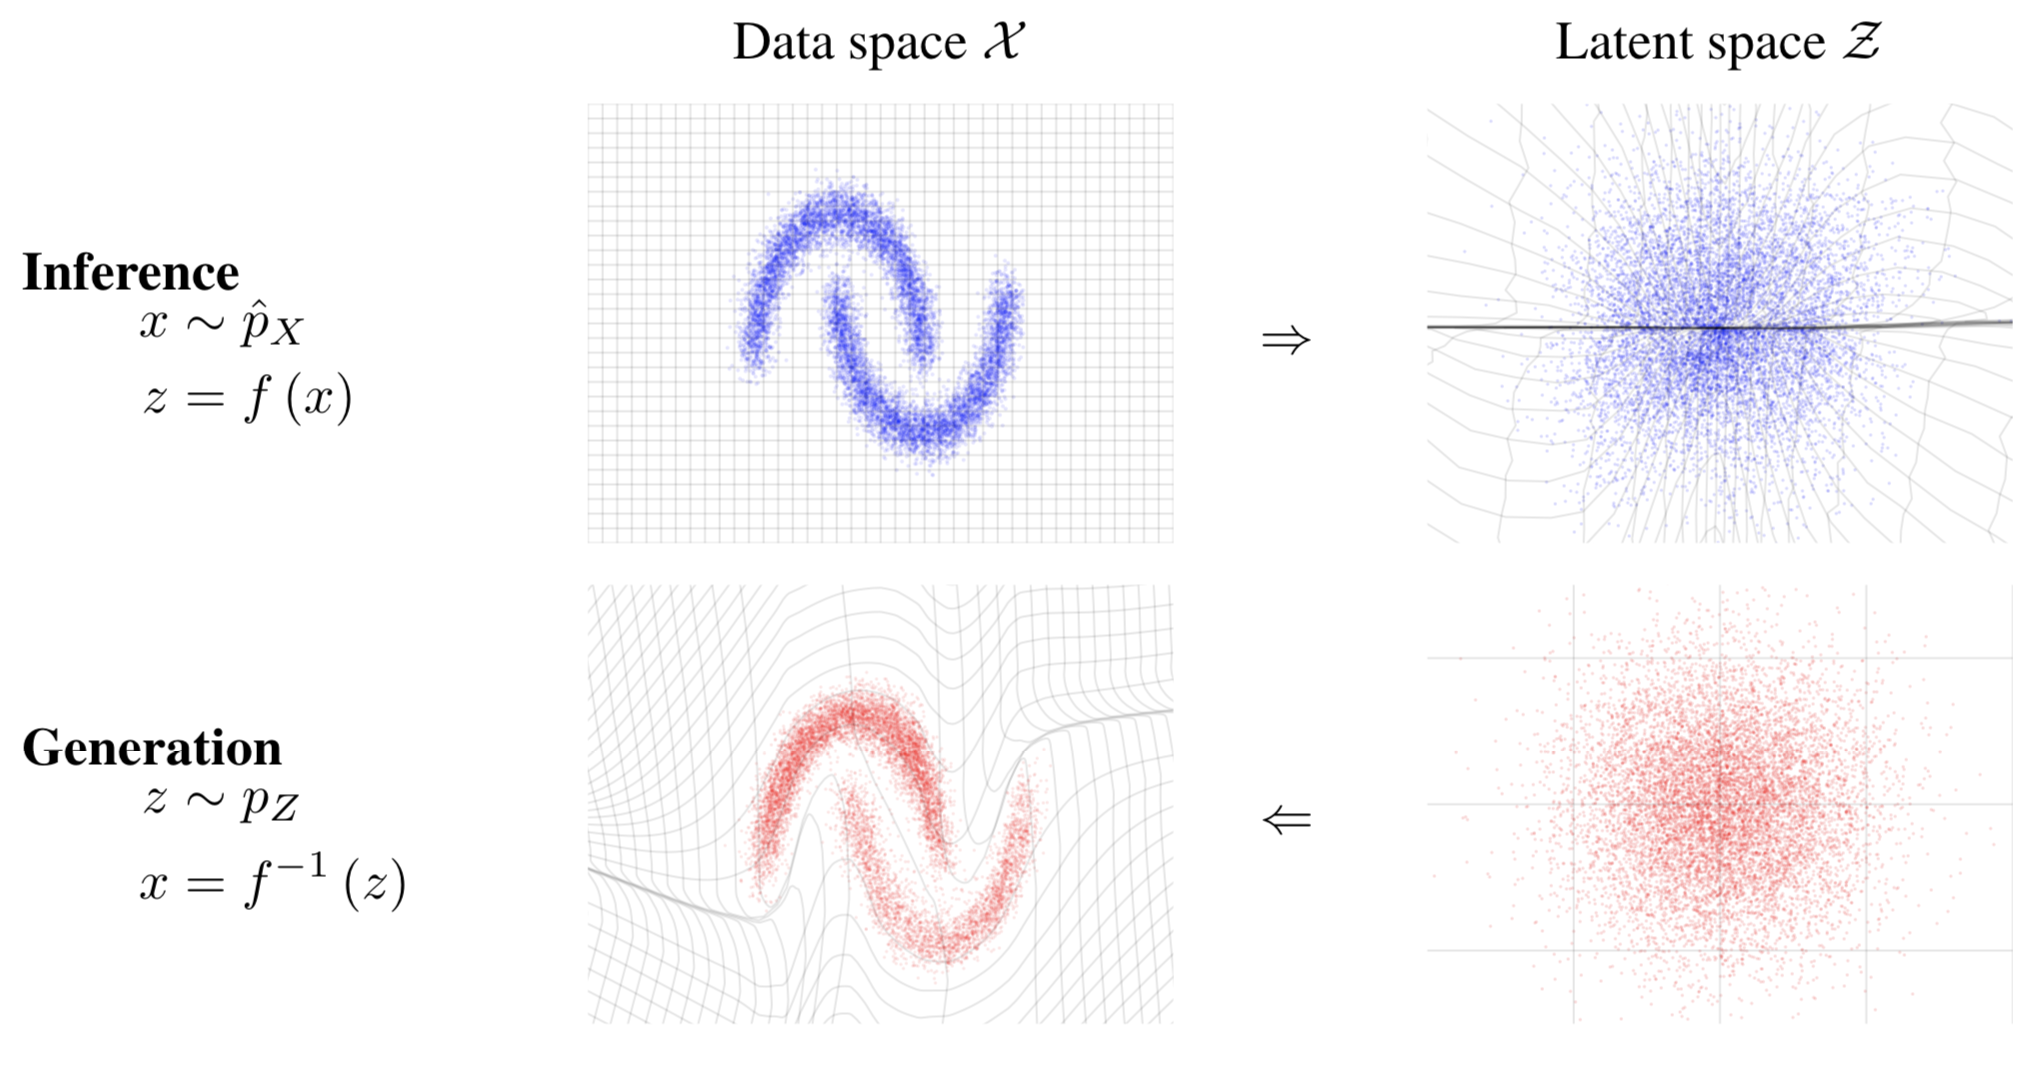
\includegraphics[width=0.85\linewidth]{figs/flows_how2}
	\end{figure}
	\vspace{-0.5cm}
	\begin{block}{Log likelihood}
		\vspace{-0.5cm}
		\[
			\log p(\bx | \btheta) = \log p(f_K \circ \dots \circ f_1(\bx)) + \sum_{k=1}^K\log |\det (\bJ_{f_k})|
		\]
	\end{block}
	\myfootnotewithlink{https://arxiv.org/abs/1605.08803}{Dinh L., Sohl-Dickstein J., Bengio S. Density estimation using Real NVP, 2016} 
\end{frame}
%=======
\begin{frame}{Recap of previous lecture}
	\begin{block}{Forward KL for flow model}
	  	\vspace{-0.1cm}
		\[
			\log p(\bx|\btheta) = \log p(f(\bx, \btheta)) + \log  |\det (\bJ_f)|
		\]
		\vspace{-0.3cm}
	\end{block}
	\begin{block}{Reverse KL for flow model}
  		\vspace{-0.5cm}
		\[
			KL(p || \pi)  = \bbE_{p(\bz)} \left[  \log p(\bz) -  \log |\det (\bJ_g)| - \log \pi(g(\bz, \btheta)) \right]
		\]
		\vspace{-0.5cm}
	\end{block}
	\begin{block}{Flow KL duality}
	  	\vspace{-0.3cm}
		\[
			\argmin_{\btheta} KL(\pi(\bx) || p(\bx | \btheta)) = \argmin_{\btheta} KL(p(\bz | \btheta) || p(\bz))
		\]
		\vspace{-0.3cm}
		\begin{itemize}
			\item $p(\bz)$ is a base distribution; $\pi(\bx)$ is a data distribution;
			\item $\bz \sim p(\bz)$, $\bx = g(\bz, \btheta)$, $\bx \sim p(\bx| \btheta)$;
			\item $\bx \sim \pi(\bx)$, $\bz = f(\bx, \btheta)$, $\bz \sim p(\bz | \btheta)$.
		\end{itemize}
	\end{block}
	\myfootnotewithlink{https://arxiv.org/abs/1912.02762}{Papamakarios G. et al. Normalizing flows for probabilistic modeling and inference, 2019} 
\end{frame}
%=======
\begin{frame}{Recap of previous lecture}
	\vspace{-0.5cm}
	\begin{block}{Flow log-likelihood}
		\vspace{-0.3cm}
		\[
			\log p(\bx|\btheta) = \log p(f(\bx, \btheta)) + \log  |\det (\bJ_f)|
		\]
		\vspace{-0.5cm}
	\end{block}
	The main challenge is a determinant of the Jacobian.
	\begin{block}{Linear flows}	
		\vspace{-0.2cm}
		\[
			\bz = f(\bx, \btheta) = \bW \bx, \quad \bW \in \bbR^{m \times m}, \quad \btheta = \bW, \quad \bJ_f = \bW^T
		\]
	\end{block}
	\vspace{-0.3cm}
	\begin{itemize}
		\item LU-decomposition
		\[
			\bW = \mathbf{P} \bL \bU.
		\]
		\item QR-decomposition
		\[
			\bW = \bQ \mathbf{R}.
		\]
	\end{itemize}
	Decomposition should be done only once in the beggining. Next, we fit decomposed matrices ($\bP/\bL/\bU$ or $\bQ/\bR$).
	\myfootnote{\href{https://arxiv.org/abs/1807.03039}{Kingma D. P., Dhariwal P. Glow: Generative Flow with Invertible 1x1 Convolutions, 2018}  \\
	\href{https://arxiv.org/abs/1901.11137}{Hoogeboom E., et al. Emerging convolutions for generative normalizing flows, 2019}
	}
\end{frame}
%=======
\begin{frame}{Outline}
	\tableofcontents
\end{frame}
%=======
\section{Autoregressive flows}
%=======
\subsection{Gaussian autoregressive flows}
%=======
\begin{frame}{Gaussian autoregressive model}
	Consider an autoregressive model
	\vspace{-0.3cm}
	{\small
		\[
		p(\bx | \btheta) = \prod_{j=1}^m p(x_j | \bx_{1:j - 1}, \btheta), \quad
		p(x_j | \bx_{1:j - 1}, \btheta) = \mathcal{N} \left(\mu_j(\bx_{1:j-1}), \sigma^2_j (\bx_{1:j-1})\right).
		\]
	}
	\vspace{-0.5cm}
	\begin{block}{Sampling: reparametrization trick}
		\vspace{-0.3cm}
		\[
		x_j = \sigma_j (\bx_{1:j-1}) \cdot z_j + \mu_j(\bx_{1:j-1}), \quad z_j \sim \mathcal{N}(0, 1).
		\]
		\vspace{-0.7cm}
	\end{block}
	\begin{block}{Inverse transform}
		\vspace{-0.3cm}
		\[
		z_j = \left(x_j - \mu_j(\bx_{1:j-1}) \right) \cdot \frac{1}{\sigma_j (\bx_{1:j-1}) }.
		\]
		\vspace{-0.4cm}
	\end{block}
	\begin{itemize}
		\item We have an \textbf{invertible} and \textbf{differentiable} transformation from $p(\bz)$ to $p(\bx | \btheta)$.
		\item It is an autoregressive (AR) flow with the base distribution $p(\bz) = \cN(0, 1)$!
		\item Jacobian of such transformation is triangular!
	\end{itemize}
	\myfootnotewithlink{https://arxiv.org/abs/1606.04934}{Kingma D. P. et al. Improving Variational Inference with Inverse Autoregressive Flow, 2016} 
\end{frame}
%=======
\begin{frame}{Gaussian autoregressive flow}
	\vspace{-0.2cm}
	\begin{align*}
		\bx &= g(\bz, \btheta) \quad \Rightarrow \quad {\color{violet} x_j} = \sigma_j ({\color{violet} \bx_{1:j-1}}) \cdot {\color{teal} z_j} + \mu_j({\color{violet} \bx_{1:j-1}}). \\
		\bz &= f(\bx, \btheta) \quad \Rightarrow \quad {\color{teal} z_j} = \left({\color{violet}x_j} - \mu_j({\color{violet}\bx_{1:j-1}}) \right) \cdot \frac{1}{ \sigma_j ({\color{violet}\bx_{1:j-1}})}.
	\end{align*}
	Generation function $g(\bz, \btheta)$ is \textbf{sequential}. \\ Inference function $f(\bx, \btheta)$ is \textbf{not sequential}.

	\begin{block}{Forward KL for NF}
		\vspace{-0.5cm}
		\[
			KL(\pi || p)  = - \bbE_{\pi(\bx)} \left[\log p(f(\bx, \btheta)) + \log  |\det (\bJ_f)|\right] + \text{const} 
		\]
		\vspace{-0.5cm}
		\begin{itemize}
			\item We need to be able to compute $f(\bx, \btheta)$ and its Jacobian.
			\item We need to be able to compute the density $p(\bz)$.
			\item We don’t need to think about computing the function $g(\bz, \btheta) = f^{-1}(\bz, \btheta)$ until we want to sample from the model.
		\end{itemize}
	\end{block}
	\myfootnotewithlink{https://arxiv.org/abs/1705.07057}{Papamakarios G., Pavlakou T., Murray I. Masked Autoregressive Flow for Density Estimation, 2017} 
\end{frame}
%=======
\subsection{Inverse gaussian autoregressive flows}
%=======
\begin{frame}{Inverse gaussian autoregressive flow (IAF)}
	Let use the following reparametrization:
	$\tilde{\bsigma} = \frac{1}{\bsigma}$; $ \tilde{\bmu} = - \frac{\bmu}{\bsigma}$.
	
	\begin{block}{Gaussian autoregressive flow}
		\vspace{-0.5cm}
		\begin{align*}
			x_j &= \sigma_j (\bx_{1:j-1}) \cdot z_j + \mu_j(\bx_{1:j-1}) =  \left( z_j - \tilde{\mu}_j(\bx_{1:j-1})\right) \cdot \frac{1}{\tilde{\sigma}_j (\bx_{1:j-1}) }\\
			z_j &= \left(x_j - \mu_j(\bx_{1:j-1}) \right) \cdot \frac{1}{ \sigma_j (\bx_{1:j-1})} = \tilde{\sigma}_j (\bx_{1:j-1}) \cdot x_j + \tilde{\mu}_j(\bx_{1:j-1}).
		\end{align*}
		\vspace{-0.3cm}
	\end{block}
	Let just swap $\bz$ and $\bx$. 
	
	\begin{block}{Inverse gaussian autoregressive flow}
		\vspace{-0.5cm}
		\begin{align*}
			\bx &= g(\bz, \btheta) \quad \Rightarrow \quad {\color{violet}x_j} = \tilde{\sigma}_j ({\color{teal}\bz_{1:j-1}}) \cdot {\color{teal} z_j} + \tilde{\mu}_j({\color{teal}\bz_{1:j-1}}) \\
			\bz &= f(\bx, \btheta) \quad \Rightarrow \quad {\color{teal}z_j} = \left( {\color{violet} x_j} - \tilde{\mu}_j({\color{teal}\bz_{1:j-1}})\right) \cdot \frac{1}{\tilde{\sigma}_j ({\color{teal}\bz_{1:j-1}}) }.
		\end{align*}
		\vspace{-0.3cm}
	\end{block}
	
	\myfootnotewithlink{https://arxiv.org/abs/1606.04934}{Kingma D. P. et al. Improving Variational Inference with Inverse Autoregressive Flow, 2016} 
\end{frame}
%=======
\begin{frame}{Inverse gaussian autoregressive flow (IAF)}
	
	\begin{minipage}[t]{0.65\columnwidth}
		\begin{block}{Gaussian autoregressive flow: $g(\bz, \btheta)$}
			\[
			x_j = \sigma_j (\bx_{1:j-1}) \cdot z_j + \mu_j(\bx_{1:j-1}).
			\]
		\end{block}
	\end{minipage}%
	\begin{minipage}[t]{0.35\columnwidth}
		\begin{figure}[h]
			\centering
			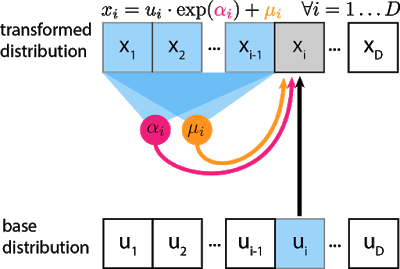
\includegraphics[width=.9\linewidth]{figs/af_iaf_explained_1.png}
		\end{figure}
	\end{minipage} \\
	
	\begin{minipage}[t]{0.65\columnwidth}
		\begin{block}{Inverse transform: $f(\bx, \btheta)$}
			\vspace{-0.5cm}
			\begin{align*}
				z_j &= (x_j - \mu_j(\bx_{1:j-1})) \cdot \frac{1}{\sigma_j (\bx_{1:j-1}) }; \\
				z_j &= \tilde{\sigma}_j (\bx_{1:j-1}) \cdot x_j + \tilde{\mu}_j(\bx_{1:j-1}).
			\end{align*}
			\vspace{-0.4cm}
		\end{block}
	\end{minipage}% 
	\begin{minipage}[t]{0.35\columnwidth}
		\begin{figure}[h]
			\centering
			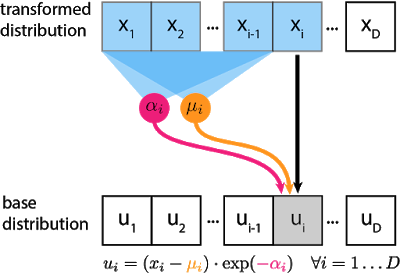
\includegraphics[width=.9\linewidth]{figs/af_iaf_explained_2.png}
		\end{figure}
	\end{minipage}\\
	\vspace{0.1cm}
	
	\begin{minipage}[t]{0.65\columnwidth}
		\begin{block}{Inverse gaussian autoregressive flow: $g(\bz, \btheta)$}
			\vspace{-0.3cm}
			\[
			x_j = \tilde{\sigma}_j (\bz_{1:j-1}) \cdot z_j + \tilde{\mu}_j(\bz_{1:j-1}).
			\]
		\end{block}
	\end{minipage}%
	\begin{minipage}[t]{0.35\columnwidth}
		\begin{figure}[h]
			\centering
			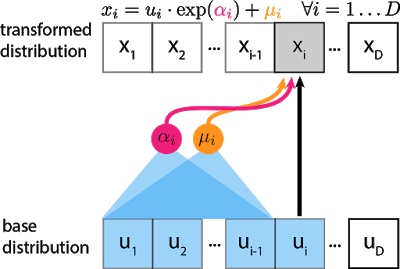
\includegraphics[width=.9\linewidth]{figs/af_iaf_explained_3.png}
		\end{figure}
	\end{minipage}
	
	\myfootnotewithlink{https://blog.evjang.com/2018/01/nf2.html}{image credit: https://blog.evjang.com/2018/01/nf2.html}
\end{frame}
%=======
\begin{frame}{Inverse gaussian autoregressive flow (IAF)}
	\begin{block}{Inverse gaussian autoregressive flow}
		\vspace{-0.5cm}
		\begin{align*}
			\bx &= g(\bz, \btheta) \quad \Rightarrow \quad {\color{violet}x_j} = \tilde{\sigma}_j ({\color{teal}\bz_{1:j-1}}) \cdot {\color{teal} z_j} + \tilde{\mu}_j({\color{teal}\bz_{1:j-1}}) \\
			\bz &= f(\bx, \btheta) \quad \Rightarrow \quad {\color{teal}z_j} = \left( {\color{violet} x_j} - \tilde{\mu}_j({\color{teal}\bz_{1:j-1}})\right) \cdot \frac{1}{\tilde{\sigma}_j ({\color{teal}\bz_{1:j-1}}) }.
		\end{align*}
		\vspace{-0.3cm}
	\end{block}
	\begin{block}{Reverse KL for NF}
		\vspace{-0.3cm}
		\[
			KL(p || \pi)  = \bbE_{p(\bz)} \left[ \log p(\bz) -  \log |\det (\bJ_g)|  - \log \pi(g(\bz, \btheta)) \right]
		\]
		\vspace{-0.3cm}
		\begin{itemize}
			\item We need to be able to compute $g(\bz, \btheta)$ and its Jacobian.
			\item We need to be able to sample from the density $p(\bz)$ (do not need to evaluate it) and to evaluate(!) $\pi(\bx)$.
			\item We don’t need to think about computing the function $f(\bx, \btheta)$.
		\end{itemize}
	\end{block}
\end{frame}
%=======
\begin{frame}{Gaussian autoregressive NF}
	\begin{block}{Gaussian AR NF}
		\vspace{-0.6cm}
		\begin{align*}
			\bx &= g(\bz, \btheta) \quad \Rightarrow \quad {\color{violet}x_j} = \sigma_j ({\color{violet}\bx_{1:j-1}}) \cdot {\color{teal} z_j} + \mu_j({\color{violet}\bx_{1:j-1}}). \\
			\bz &= f(\bx, \btheta) \quad \Rightarrow \quad {\color{teal} z_j} = \left({\color{violet} x_j} - \mu_j({\color{violet}\bx_{1:j-1}}) \right) \cdot \frac{1}{\sigma_j ({\color{violet} \bx_{1:j-1}}) }.
		\end{align*}
		\vspace{-0.6cm}
		\begin{itemize}
			\item Sampling is sequential, density estimation is parallel.
			\item Forward KL is a natural loss.
		\end{itemize}
	\end{block}
	\begin{block}{Inverse gaussian AR NF}
		\vspace{-0.6cm}
		\begin{align*}
			\bx &= g(\bz, \btheta) \quad \Rightarrow \quad {\color{violet} x_j} = \tilde{\sigma}_j ({\color{teal}\bz_{1:j-1}}) \cdot {\color{teal} z_j} + \tilde{\mu}_j({\color{teal}\bz_{1:j-1}}) \\
			\bz &= f(\bx, \btheta) \quad \Rightarrow \quad {\color{teal}z_j} = \left( {\color{violet} x_j} - \tilde{\mu}_j({\color{teal}\bz_{1:j-1}})\right) \cdot \frac{1}{\tilde{\sigma}_j ({\color{teal}\bz_{1:j-1}}) }.
		\end{align*}
		\vspace{-0.6cm}
		\begin{itemize}
			\item Sampling is parallel, density estimation is sequential.
			\item Reverse KL is a natural loss.
		\end{itemize}
	\end{block}
	\myfootnotewithlink{https://arxiv.org/abs/1606.04934}{Kingma D. P. et al. Improving Variational Inference with Inverse Autoregressive Flow, 2016} 
\end{frame}
%=======
\begin{frame}{Autoregressive flows}
	Gaussian AR NF and inverse gaussian AR NF are mutually interchangeable. 
	\begin{figure}
		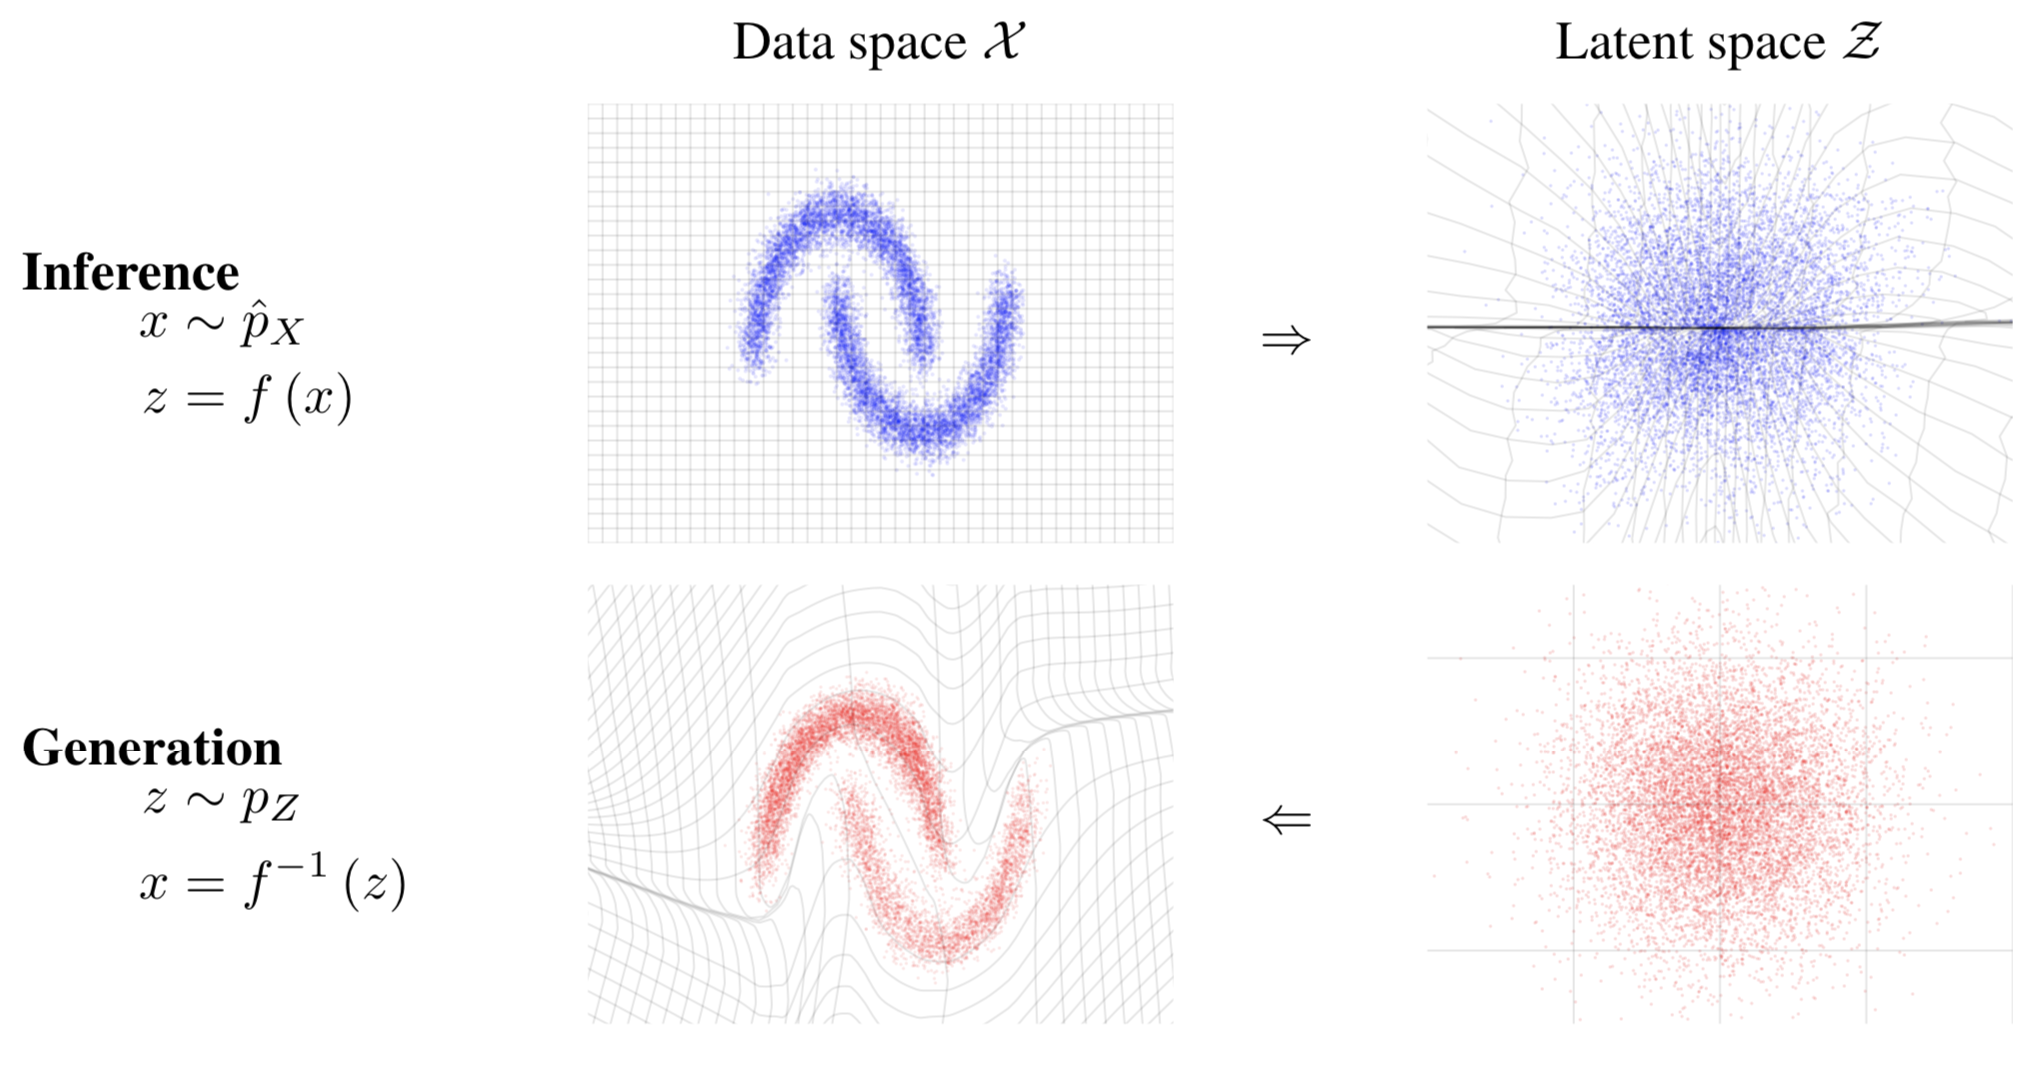
\includegraphics[width=\linewidth]{figs/flows_how2.png}
	\end{figure}
	
	\myfootnotewithlink{https://arxiv.org/abs/1605.08803}{Dinh L., Sohl-Dickstein J., Bengio S. Density estimation using Real NVP, 2016} 
\end{frame}
%=======
\subsection{RealNVP: coupling layer}
%=======
\begin{frame}{RealNVP}
	\vspace{-0.5cm}
	Let split $\bx$ and $\bz$ in two parts: 
	\[
		\bx = [\bx_1, \bx_2] = [\bx_{1:d}, \bx_{d+1:m}]; \quad \bz = [\bz_1, \bz_2] = [\bz_{1:d}, \bz_{d+1:m}].
	\]
	\vspace{-0.7cm}
	\begin{block}{Coupling layer}
		\vspace{-0.7cm}
		\[
			\begin{cases} \bx_1 = \bz_1; \\ \bx_2 = \bz_2 \odot \bsigma(\bz_1, \btheta) + \bmu(\bz_1, \btheta).\end{cases}  
			\begin{cases} \bz_1 = \bx_1; \\ \bz_2 = \left(\bx_2 - \bmu({\color{olive}\bx_1}, \btheta) \right) \odot \frac{1}{\bsigma({\color{olive}\bx_1}, \btheta)}.\end{cases}
		\]
	\end{block}
	\vspace{-0.5cm}
	\begin{block}{Image partitioning}
		
		\begin{minipage}[t]{0.5\columnwidth}
			\begin{figure}
				\centering
				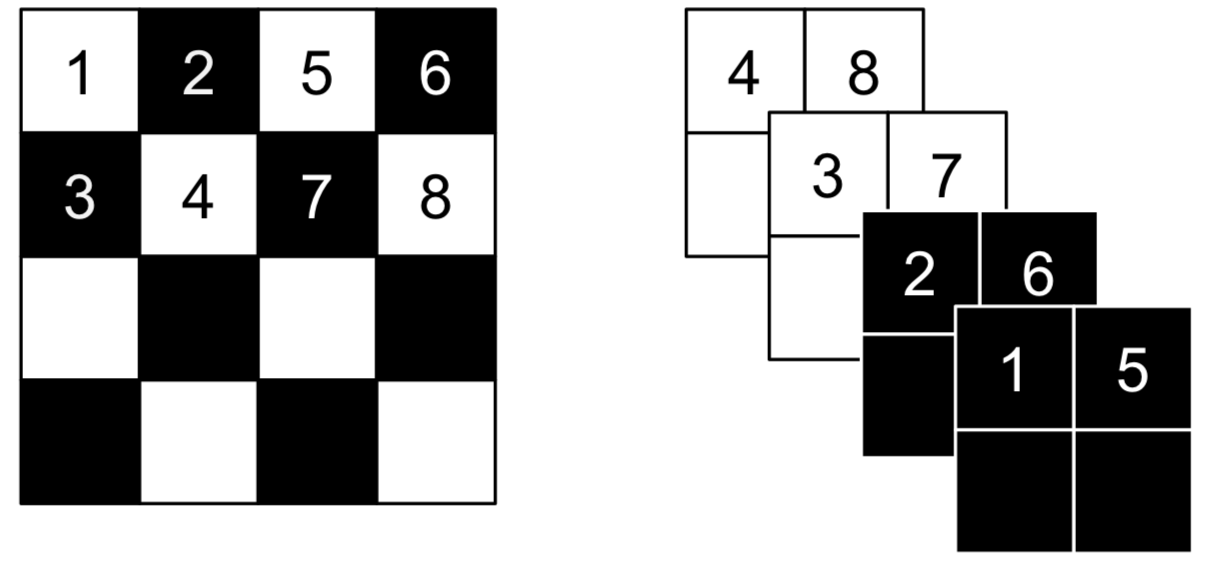
\includegraphics[width=\linewidth]{figs/realnvp_masking.png}
			\end{figure}
		\end{minipage}% 
		\begin{minipage}[t]{0.5\columnwidth}
			\begin{itemize}
				\item Checkerboard ordering uses masking.
				\item Channelwise ordering uses splitting.
			\end{itemize}
		\end{minipage}
	\end{block}
	\vspace{-0.5cm}
	\myfootnotewithlink{https://arxiv.org/abs/1605.08803}{Dinh L., Sohl-Dickstein J., Bengio S. Density estimation using Real NVP, 2016} 
\end{frame}
%=======
\begin{frame}{RealNVP}
	\begin{block}{Coupling layer}
		\vspace{-0.7cm}
		\[
		 \begin{cases} {\color{violet}\bx_1} = {\color{teal}\bz_1}; \\ {\color{violet}\bx_2} = {\color{teal}\bz_2} \odot \bsigma({\color{teal}\bz_1}, \btheta) + \bmu({\color{teal}\bz_1}, \btheta).\end{cases}  
		\begin{cases} {\color{teal}\bz_1} ={\color{violet} \bx_1}; \\ {\color{teal}\bz_2} = \left({\color{violet}\bx_2} - \bmu({\color{violet}\bx_1}, \btheta) \right) \odot \frac{1}{\bsigma({\color{violet}\bx_1}, \btheta)}.\end{cases}
		\]
		Estimating the density takes 1 pass, sampling takes 1 pass!
	\end{block}
	\begin{block}{Jacobian}
		\vspace{-0.5cm}
		\[
		\det \left( \frac{\partial \bz}{\partial \bx} \right) = \det 
		\begin{pmatrix}
			\bI_d & 0_{d \times m - d} \\
			\frac{\partial \bz_2}{\partial \bx_1} & \frac{\partial \bz_2}{\partial \bx_2}
		\end{pmatrix} = \prod_{j=1}^{m - d} \frac{1}{\sigma_j(\bx_1, \btheta)}.
		\]
		\vspace{-0.5cm}
	\end{block}
	\begin{block}{Gaussian AR NF}
		\vspace{-0.6cm}
		\begin{align*}
			\bx &= g(\bz, \btheta) \quad \Rightarrow \quad {\color{violet}x_j} = \sigma_j ({\color{violet}\bx_{1:j-1}}) \cdot {\color{teal} z_j} + \mu_j({\color{violet}\bx_{1:j-1}}). \\
			\bz &= f(\bx, \btheta) \quad \Rightarrow \quad {\color{teal} z_j} = \left({\color{violet} x_j} - \mu_j({\color{violet}\bx_{1:j-1}}) \right) \cdot \frac{1}{\sigma_j ({\color{violet} \bx_{1:j-1}}) }.
		\end{align*}
		\vspace{-0.5cm}
	\end{block}
	How to get RealNVP coupling layer from gaussian AR NF?
	
	\myfootnotewithlink{https://arxiv.org/abs/1605.08803}{Dinh L., Sohl-Dickstein J., Bengio S. Density estimation using Real NVP, 2016} 
\end{frame}
%=======
\begin{frame}{Glow samples}
	Glow model: coupling layer + linear flows (1x1 convs)
	\begin{figure}
		\centering
		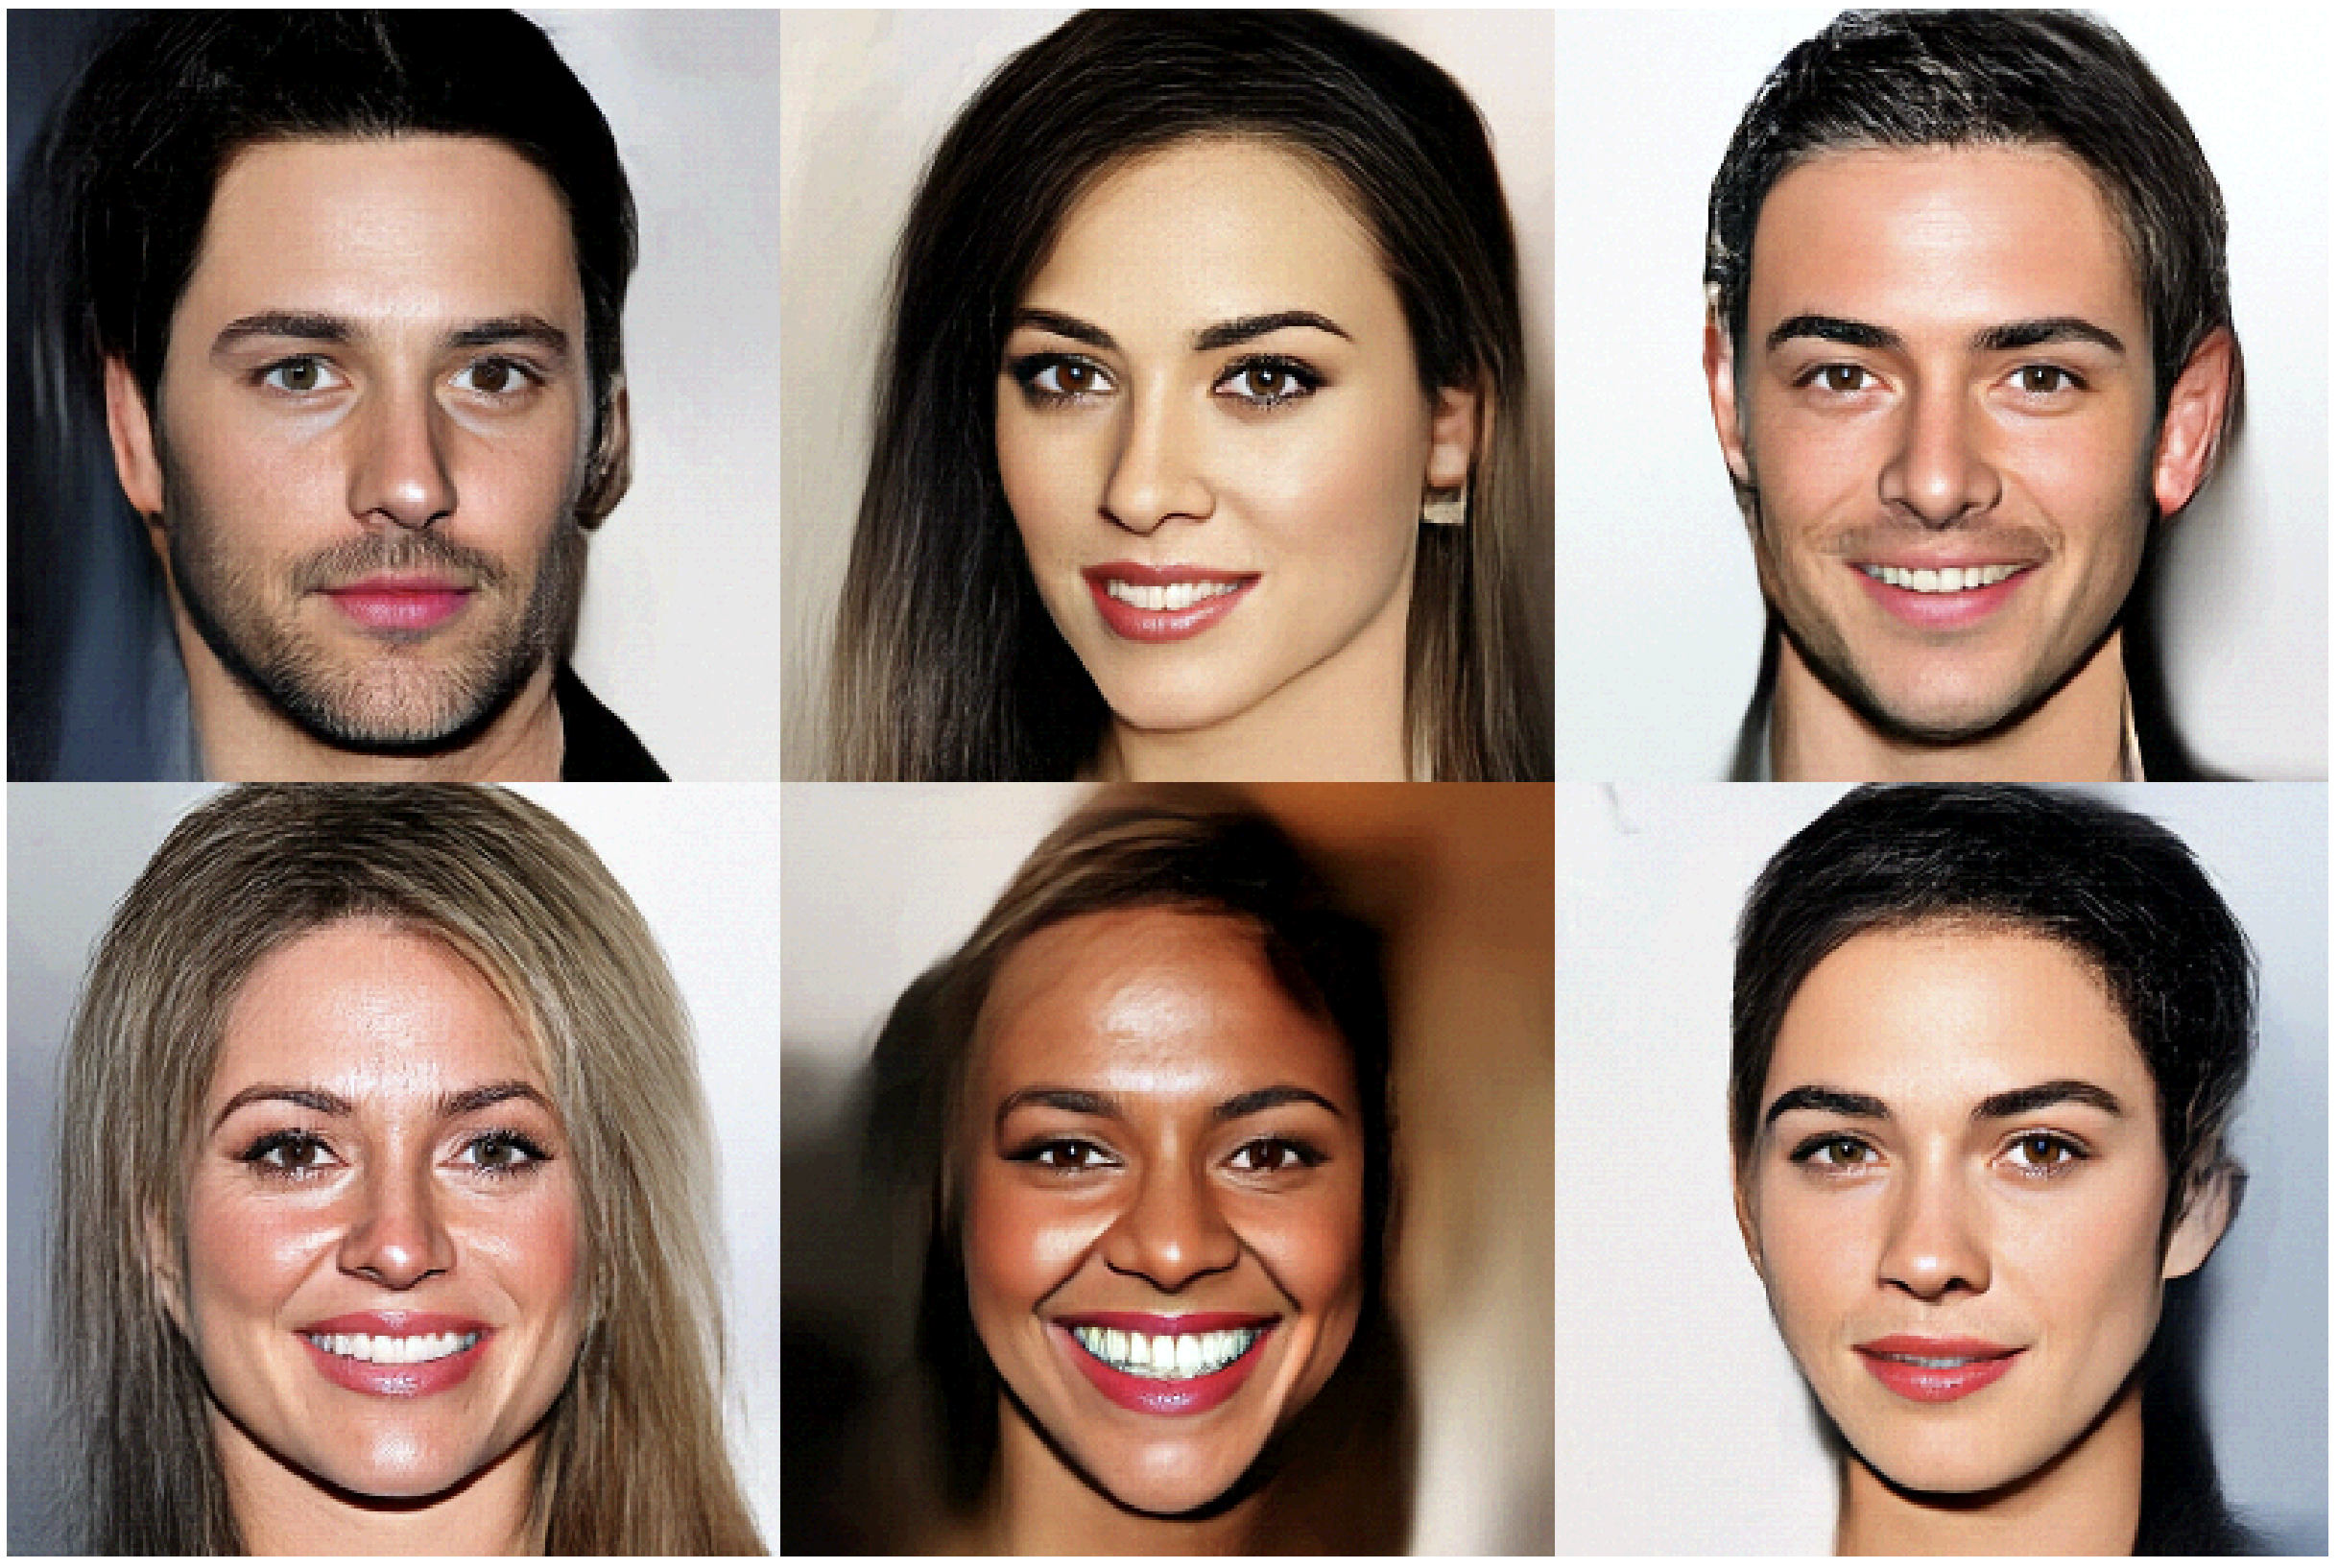
\includegraphics[width=0.9\linewidth]{figs/glow_faces.png}
	\end{figure}
	\myfootnotewithlink{https://arxiv.org/abs/1807.03039}{Kingma D. P., Dhariwal P. Glow: Generative Flow with Invertible 1x1 Convolutions, 2018}
\end{frame}
%=======
\begin{frame}{Venn diagram for Normalizing flows}
	
	\begin{figure}
		\centering
		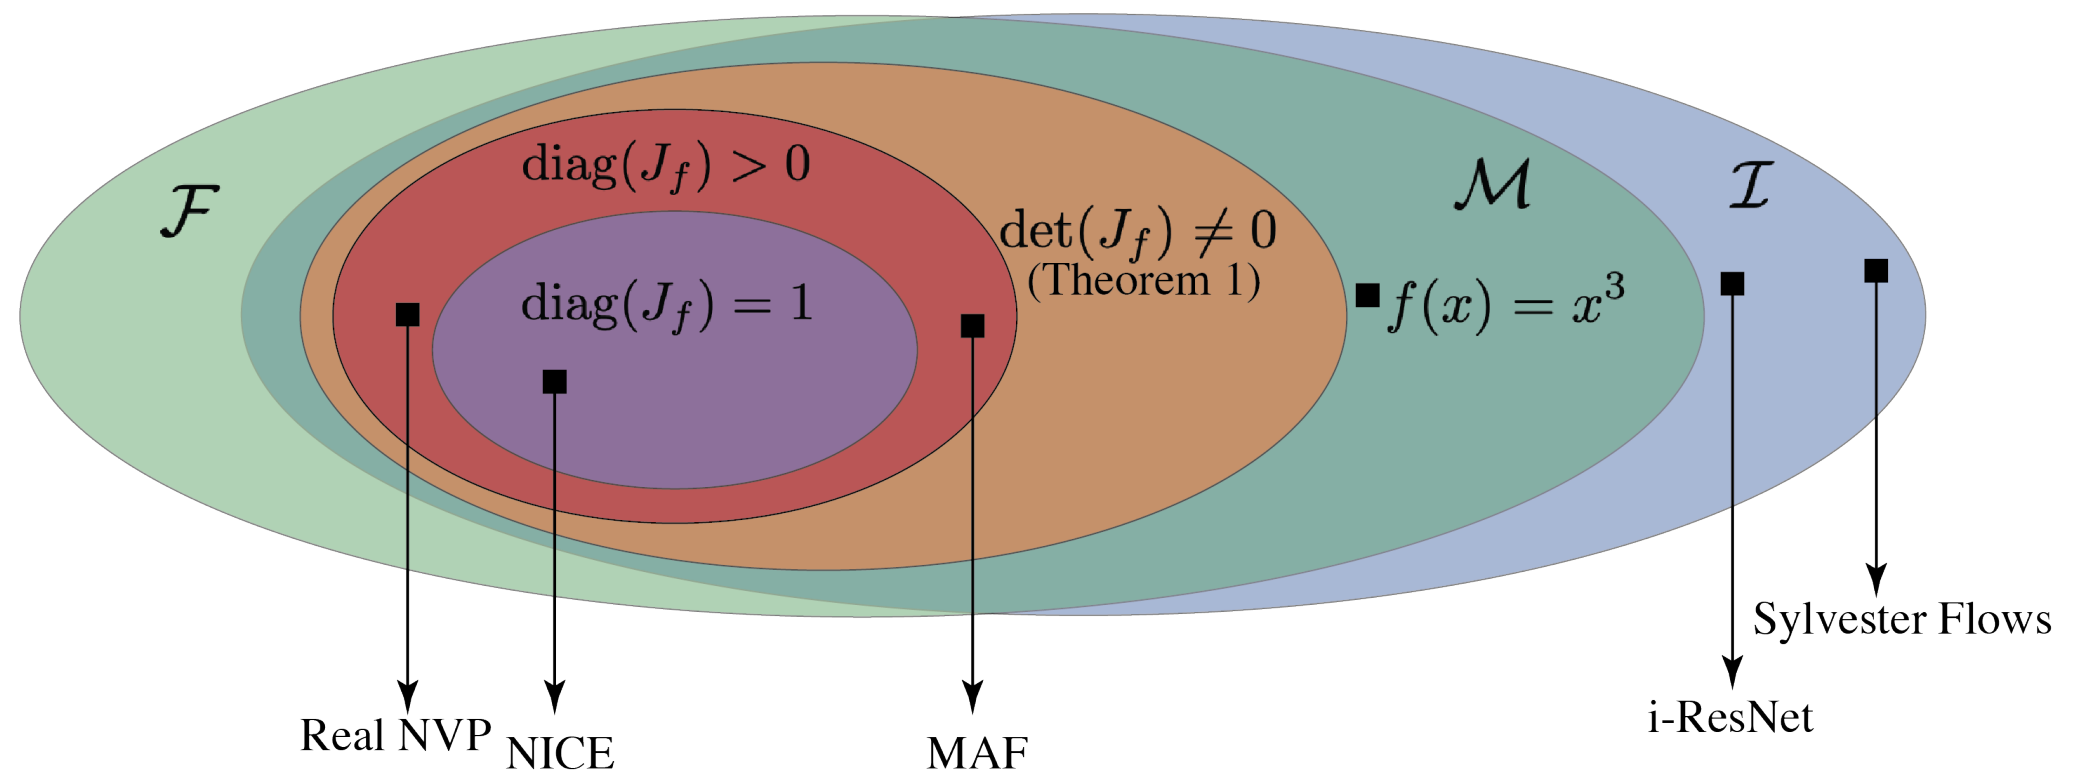
\includegraphics[width=\linewidth]{figs/venn_diagram}
	\end{figure}
	\begin{itemize}
		\item $\cI$ -- invertible functions.
		\item $\cF$ -- continuously differentiable functions whose Jacobian is lower triangular.
		\item $\cM$ -- invertible functions from $\cF$.
	\end{itemize}
	\myfootnotewithlink{https://arxiv.org/abs/1907.07945}{Song Y., Meng C., Ermon S. Mintnet: Building invertible neural networks with masked convolutions, 2019}
\end{frame}
%=======
\section{Normalizing flows as VAE model}
%=======
\begin{frame}{VAE vs Normalizing flows}
	\begin{table}[]
		\begin{tabular}{l|c|c}
			& \textbf{VAE} & \textbf{NF} \\ \hline
			\textbf{Objective} & ELBO $\cL$ & Forward KL/MLE \\ \hline
			\textbf{Encoder} & \shortstack{stochastic \\ $\bz \sim q (\bz | \bx, \bphi)$} &  \shortstack{\\ deterministic \\ $\bz = f(\bx, \btheta)$ \\ $q(\bz | \bx, \btheta) = \delta(\bz - f(\bx, \btheta))$}  \\ \hline
			\textbf{Decoder} & \shortstack{stochastic \\ $\bx \sim p (\bx | \bz, \btheta)$} & \shortstack{\\ deterministic \\ $\bx = g(\bz, \btheta)$ \\ $ p(\bx | \bz, \btheta) = \delta(\bx - g(\bz, \btheta))$} \\ \hline
			\textbf{Parameters}  & $\bphi, \btheta$ & $\btheta \equiv \bphi$\\ 
		\end{tabular}
	\end{table}
	\begin{block}{Theorem}
		MLE for normalizing flow is equivalent to maximization of ELBO for VAE model with deterministic encoder and decoder:
		\vspace{-0.3cm}
		\[
			p(\bx | \bz, \btheta) = \delta (\bx - f^{-1}(\bz, \btheta)) = \delta (\bx - g(\bz, \btheta));
		\]
		\[
			q(\bz | \bx, \btheta) = p(\bz | \bx, \btheta) = \delta (\bz - f(\bx, \btheta)).
		\]
	\end{block}
	\myfootnotewithlink{https://arxiv.org/abs/2007.02731}{Nielsen D., et al. SurVAE Flows: Surjections to Bridge the Gap between VAEs and Flows, 2020}
\end{frame}
%=======
\begin{frame}{Normalizing flow as VAE}
	\begin{block}{Proof}
		\begin{enumerate}
			\item Dirac delta function property 
			\[
				\bbE_{\delta(\bx - \by)} f(\bx) d \bx = \int \delta(\bx - \by) f(\bx) d \bx = f(\by).
			\]
			\item CoV theorem and Bayes theorem:
			\[
				p(\bx | \btheta) = p(\bz) |\det (\bJ_f)|;
			\]
			\[
				p(\bz | \bx, \btheta) = \frac{p(\bx | \bz, \btheta) p(\bz)}{p(\bx | \btheta)}; \quad \Rightarrow \quad p(\bx | \bz, \btheta) = p(\bz | \bx, \btheta) |\det (\bJ_f)|.
			\]
			\item Log-likelihood decomposition
			\[
				\log p(\bx | \btheta) = \cL(\btheta) + {\color{olive}KL(q(\bz | \bx, \btheta) || p(\bz | \bx, \btheta))} = \cL(\btheta).
			\]
		\end{enumerate}
	\end{block}
	\myfootnotewithlink{https://arxiv.org/abs/2007.02731}{Nielsen D., et al. SurVAE Flows: Surjections to Bridge the Gap between VAEs and Flows, 2020}
\end{frame}
%=======
\begin{frame}{Normalizing flow as VAE}
	\begin{block}{Proof}
		ELBO objective:
		\vspace{-0.5cm}
		\begin{multline*}
			\cL  = \bbE_{q(\bz | \bx, \btheta)} \left[\log p(\bx | \bz, \btheta) - \log \frac{q(\bz | \bx, \btheta)}{p(\bz)} \right]  \\
			= \bbE_{q(\bz | \bx, \btheta)} \left[{\color{violet}\log \frac{p(\bx | \bz, \btheta)}{q(\bz | \bx, \btheta)}} + {\color{teal}\log p(\bz)} \right].
		\end{multline*}
		\vspace{-0.6cm}
		\begin{enumerate}
			\item  Dirac delta function property:
			\vspace{-0.3cm}
			\[
				{\color{teal}\bbE_{q(\bz | \bx, \btheta)} \log p(\bz)} = \int \delta (\bz - f(\bx, \btheta)) \log p(\bz) d \bz = \log p(f(\bx, \btheta)).
			\]
			\vspace{-0.6cm}
			\item CoV theorem and Bayes theorem:
			\vspace{-0.2cm}
			{ \small
			\[ 
				{\color{violet}\bbE_{q(\bz | \bx, \btheta)} \log \frac{p(\bx | \bz, \btheta)}{q(\bz | \bx, \btheta)}} = \bbE_{q(\bz | \bx, \btheta)} \log \frac{p(\bz | \bx, \btheta) |\det (\bJ_f)|}{q(\bz | \bx, \btheta)} = \log |\det \bJ_f|.
			\]
			}
			\vspace{-0.6cm}
			\item Log-likelihood decomposition
			\vspace{-0.3cm}
			\[
				\log p(\bx | \btheta) = \cL(\btheta) = \log p(f(\bx, \btheta)) +  \log |\det \bJ_f|.
			\]
		\end{enumerate}
	\end{block}
	\myfootnotewithlink{https://arxiv.org/abs/2007.02731}{Nielsen D., et al. SurVAE Flows: Surjections to Bridge the Gap between VAEs and Flows, 2020}
\end{frame}
%=======
\begin{frame}{Summary}
	\begin{itemize}
		\item Gaussian autoregressive flow is an autoregressive model with triangular Jacobian. It has fast inference function and slow generation function. Forward KL is a natural loss function.
		\vfill
		\item Inverse gaussian autoregressive flow generate new samples fast, but the inference is slow. Reverse KL is a natural loss function.
		\vfill
		\item The RealNVP coupling layer is an effective type of flow (special case of AR flows) that has fast inference and generation modes.
		\vfill
		\item NF models could be treated as VAE model with deterministic encoder and decoder.
	\end{itemize}
\end{frame}
%=======
\end{document} 